\documentclass[10pt]{article}
\usepackage[breaklinks=true]{hyperref}
\usepackage[margin=0.75in]{geometry}

\usepackage{color}
\usepackage{graphicx}
\definecolor{pblue}{rgb}{0.13,0.13,1}
\definecolor{pgreen}{rgb}{0,0.5,0}
\definecolor{pred}{rgb}{0.9,0,0}
\definecolor{pgrey}{rgb}{0.46,0.45,0.48}

\usepackage{listings}
\lstset{language=bash,
	 showspaces=false,
	 showtabs=false,
	breaklines=true,
	 showstringspaces=false,
	 tabsize=2,
 breakatwhitespace=true,
	commentstyle=\color{pgreen}, keywordstyle=\color{pblue},
	stringstyle=\color{pred}, numbers=left, stepnumber=1,
	basicstyle=\small\ttfamily, frame=single, moredelim=[il][\textcolor{pgrey}]{$$},
	moredelim=[is][\textcolor{pgrey}]{\%\%}{\%\%} }

\title{\textbf{Week 13} \\
\Large Final Exam Prep \& Closing Remarks}
\author{ Melvyn Ian Drag }
\date{\today}

\begin{document}
\maketitle

\begin{abstract}
Tonight we will practice for the final exam. Then we will look at a couple of
final Linux topics that we haven't had time for yet.
\end{abstract}

\section{Link for setting up gitlab on digital ocean.}
\url{https://www.youtube.com/watch?v=QCZl0eNzMTs}

\section{Final Exam Problem Statement and Motivation} 
\subsection{The Scenario}
\begin{enumerate}
\item You are an employee at a company writing software on a laptop.
\item You need to backup your code using git.
\item Your company doesn't trust github because your code is secret and cannot
be on the internet
\item Therefore you must create a git server on a Linux machine the company
controls.
\item You need to configure the server such that 
\begin{itemize}
\item You can push code from your laptop to the server
\item Your colleague can clone code from the server to his laptop
\end{itemize}
\end{enumerate}

\subsection{The Final Exam}
The problem we will do is you will need to create two fresh Digital ocean
servers in class. One will emulate your laptop described in the scenario above (
we will refer to this as the `git client').
The other will represent the company git server ( we will refer to this as the
`git server'). You need to configure the git server such that you can push a
repo from the client to the server. Then, I need you to add my laptop's
id\_rsa.pub key to your git server's authorized\_keys file so that I can clone
the repo from there.

If you practice you can complete this exam in 5 minutes. If you don't practice
you will likely be unable to complete the task. Make sure you practice, this
assignment is pass/fail, 0/100.

\section{How to do it}
\subsection{Create two Digital Ocean Debian 10 VMs}
If time, put pictures here of the vm creation.

\subsection{Configure the Server}

We need to install some software, add a special user, and create an empty git
repo to store our code.
\begin{lstlisting}
root@digitalocean-gitserver$ apt update
root@digitalocean-gitserver$ apt install git-core curl
root@digitalocean-gitserver$ adduser git
#answer questions
root@digitalocean-gitserver$ su - git
git@digitalocean-gitserver$
git@digitalocean-gitserver$ cd
git@digitalocean-gitserver$ pwd
#/home/git
git@digitalocean-gitserver$ git init --bare final_exam.git
\end{lstlisting}

We will need the ip address of this machine when we use it as a remote. Remember
that up until this point we have been using github as our remote - now we are
setting up our OWN git server. We don't need github now, because we are making
our OWN github. For now, just figure out the ipaddress of your server.

\begin{lstlisting}
git@digitalocean-gitserver$ curl ipinfo.io/ip
111.222.333.444
\end{lstlisting}


\subsection{Configure the client}
Install necessary things. 

Create a repo

Create ssh keys

\begin{lstlisting}
root@digitalocean-gitclient$ apt update
root@digitalocean-gitclient$ apt install git
root@digitalocean-gitclient$ adduser ashketchum
root@digitalocean-gitclient$ su - ashketchum
\end{lstlisting}

Now create some code,
\begin{lstlisting}
ashketchum@digitalocean-gitclient$ cd
ashketchum@digitalocean-gitclient$ pwd
/home/ashketchum
ashketchum@digitalocean-gitclient$ mkdir FinalExamCode
ashketchum@digitalocean-gitclient$ cd FinalExamCode
ashketchum@digitalocean-gitclient$ vim mycode.sh
# add some stuff to the file.
ashketchum@digitalocean-gitclient$ cat mycode.sh
echo 'hello world!'
\end{lstlisting}

Then configure your local git repository.
\begin{lstlisting}
ashketchum@digitalocean-gitclient$ pwd
/home/ashketchum/FinalExamCode
ashketchum@digitalocean-gitclient$ git config --global user.email
"ash@pallet.town"
ashketchum@digitalocean-gitclient$ git config --global user.name "Ash Ketchum"
ashketchum@digitalocean-gitclient$git init
ashketchum@digitalocean-gitclient$git add mycode.sh
ashketchum@digitalocean-gitclient$git status
# shows added code not yet committed
ashketchum@digitalocean-gitclient$git commit -m "first commit"
ashketchum@digitalocean-gitclient$git status
#shows your code is committed
ashketchum@digitalocean-gitclient$git remote add origin
git@111.222.333.444:final_exam.git
# Put the ipaddress of the machine digitalocean-gitserver.
# remember that we got the ipaddress before.
\end{lstlisting}

Now create an ssh key you can use when pushing your code the the server.
\begin{lstlisting}
ashketchum@digitalocean-gitclient$ ssh-keygen
# does stuff.
ashketchum@digitalocean-gitclient$ cat ~/.ssh/id_rsa.pub
ssh-rsa 1hd+alkhgienalX1222 ashketchum@digitalocean-gitclient
ashketchum@digitalocean-gitclient$ # you will need to paste that key in the
authorized_keys file on your git server.
\end{lstlisting}

Now we will put this key on our server. You can try to push your code to the
server now, but you will see it will fail. The key is not on the machine so it
won't work.

\begin{lstlisting}
ashketchum@digitalocean-gitclient$ pwd
/home/ashketchum/FinalExamCode
ashketchum@digitalocean-gitclient$git push origin master
# NOPE
\end{lstlisting}

\subsection{Put your ssh key on digitalocean-gitserver}

Put the key there however you wish. Copying from \textit{digitalocean-gitclient} and pasting it into the
\textit{/home/git/.ssh/authorized\_keys} file on \textit{digitalocean-gitserver} is probably easiest.

\begin{lstlisting}
git@digitalocean-gitserver$ mkdir ~/.ssh
git@digitalocean-gitserver$ touch ~/.ssh/authorized_keys
git@digitalocean-gitserver$ # now put the key in that file however you wish.
git@digitalocean-gitserver$ cat ~/.ssh/authorized_keys
ssh-rsa 1hd+alkhgienalX1222 ashketchum@digitalocean-gitclient
\end{lstlisting}

\subsection{Push to the server}
Go back on the client and push your code. It should work now!

\begin{lstlisting}
ashketchum@digitalocean-gitclient$ pwd
/home/ashketchum/FinalExamCode
ashketchum@digitalocean-gitclient$git push origin master
# This time it works.
\end{lstlisting}

\subsection{Back to the final exam.}
For the final exam, I want to be able to clone your code to my laptop. Now the
code is sitting there on the \textit{digitalocean-gitserver} machine. If you put
my ssh key from my laptop on the server, I should be able to clone the code. If
I can successfully clone the code, you get a 100. My ssh key will be provided
during the exam. 

I will try to clone your code by running ( from my laptop ):
\begin{lstlisting}
melvyn@laptop$ git clone git@111.222.333.444:final_exam.git
\end{lstlisting}

\begin{center}
{\LARGE Have students share their id\_rsa.pubs and clone each others repos. For
example, have `Mike' give `Tiffany' the contents of his id\_rsa.pub and have
here put it in the authorized\_keys file on her \textit{digitalocean-gitserver}}.
Then have him attempt to clone her code.
\end{center}

And then one more detail.



\subsection{Further reading}
This is only one way to set up a git server. There are at least a few other
ways, and there are still many questions you might have about git - now you need
to go RTFM. We've been using git and github for a few months, and now you've
even set up a server. You can now confidently pick up \textit{the book} and read
it and learn more details about this extremely complex program. Here is
\textit{the book} online for free, but you can also order the paperback off
amazon if you like that better.

\begin{center}
\url{https://git-scm.com/book/en/v2}
\end{center}

in particular you are probably interested in the section about setting up git
servers:

\begin{center}
\url{https://git-scm.com/book/en/v2/Git-on-the-Server-The-Protocols}
\end{center}
\section{Gitlab}

You will see that what the notes above described is setting up git to use the
SSH Protocol ( hence why you have to put you ssh key on the server ). That
section of the book describes some other protocols you could use for your git
server.

\section{Important Reminder!}
This is your final exam. 

\begin{enumerate}
\item We've just done it together
\item I've written quite thorough notes documenting the procedure.
\item If you don't like my writing style, I've also given you a link to the
 reference book these notes are based on. 
\item You have 2 weeks to study before the exam
\end{enumerate}

{\LARGE\textbf{A few people came to the midterm underprepared. I gave an
extension for that. There are NO extensions for the final exam. I wont answer
any questions or troubleshoot any problems during the exam - YOU have to study
and master this little bit of information. Practice this a
couple of times at home until you can do the whole process in 5 minutes, then
come in and get an easy A.} We meet at 8PM, I'm hoping that we can all be done
in a half hour and go home early.}

\section{Setting up a GitLab Server}

Before we setup a git server that works exclusively through the command line
interface. Github is a git server and you get a pretty UI with lots of buttons
on the internet. Do you like that better?

Interestingly enough you can create your own github-like website using GitLab.
Have a look at ~\ref{fig:gitlab} to see the website you'll make in the next few
minutes. You can set up this website on a PC or raspberry pi at home. Or you can
set up a cloud server on digital ocean ( or AWS or google cloud or whatever )
and run your gitlab website there. It will only be accessible to people with
login credentials, so you can use it yourself or share it with friends and
family or maybe your college buddies you get together with to write code.

\begin{figure}[h]
\centering
	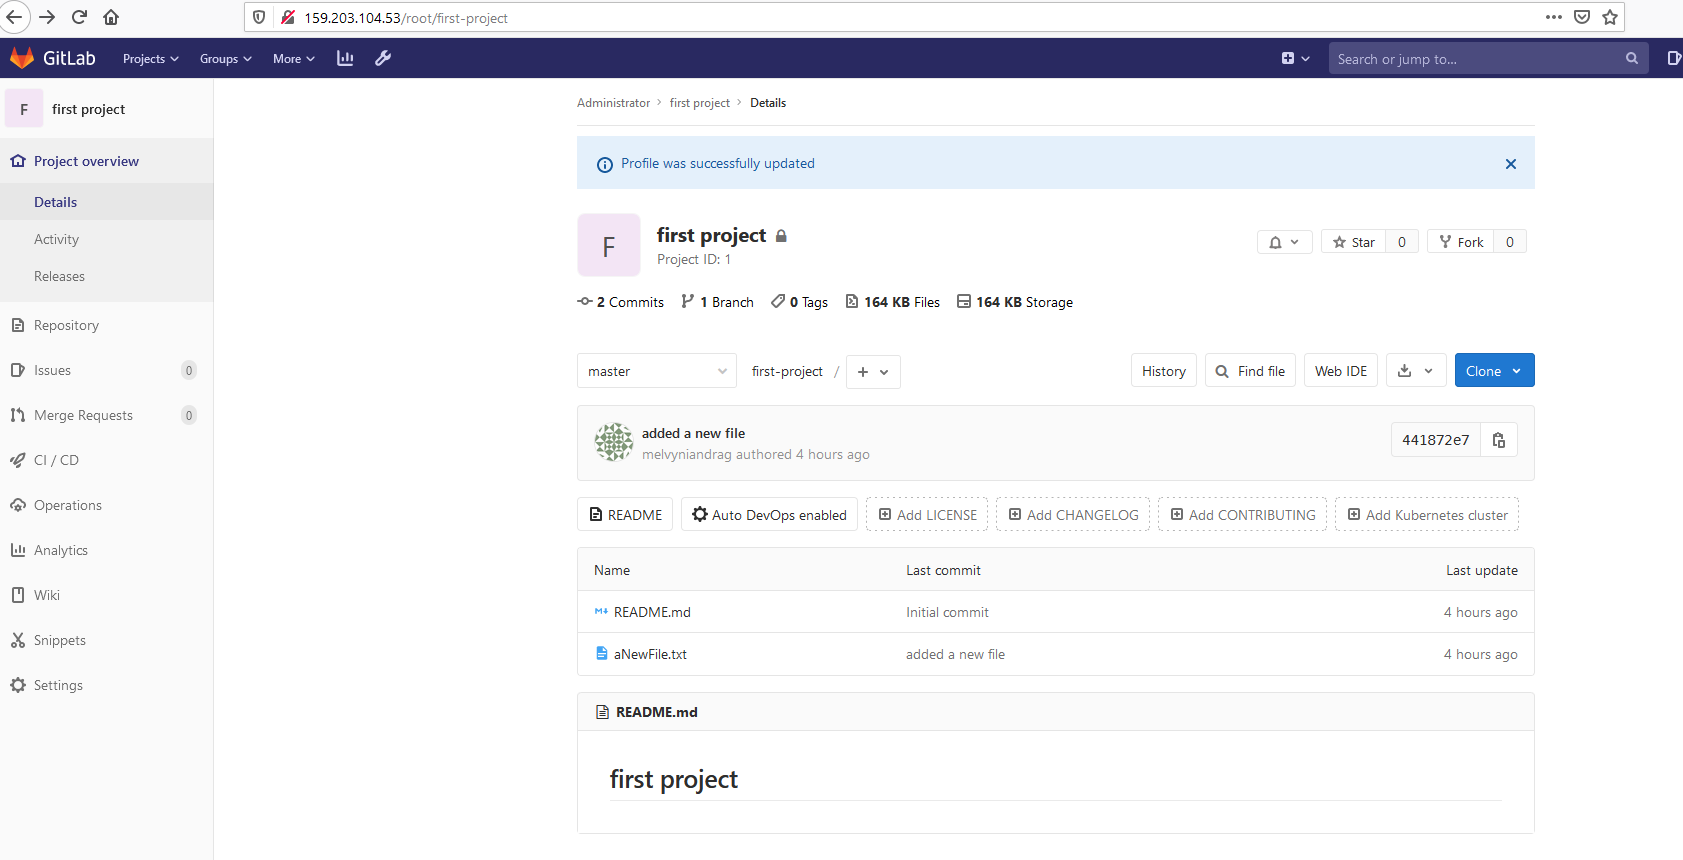
\includegraphics[width=0.8\textwidth]{Images/gitlab.PNG}
	\caption{{\small \texttt{Example of gitlab on digital ocean webserver.}}}
	\label{fig:gitlab}
\end{figure}

\subsection{Setup}
All these notes are based on information I found here:

\url{https://computingforgeeks.com/how-to-install-and-configure-gitlab-ce-on-debian-buster/}

Information always disappears from the internet. Also these notes dont work
100\%. So I'm fixing them up such that they work on Debian10 on Digital Ocean as
of 4/25/2020. If you use Ubuntu18 on AWS in 2021 I can't guarantee these notes
will work.

Also note:

You need lots of memory for this! Up until now we've been using \$5 servers that
only have 1GB of memory. According to the Gitlab requirements shown here:

\url{https://docs.gitlab.com/ee/install/requirements.html} we need 8GB of
memory. So I'm going to select a \$40 machine that has 8GB of ram. Make sure to
delete this droplet AS SOON as you finish the assignment. This way you'll spend
under 50 cents. If you leave it on, you'll run up a big charge.



Do the following:

\begin{lstlisting}
root@server$ apt update
root@server$ apt -y install curl gnupg2 ca-certificates
root@server$ curl https://packages.gitlab.com/install/repositories/gitlab/gitlab-ce/script.deb.sh | sudo bash
\end{lstlisting}

At this point you should see:

\begin{lstlisting}
The repository is setup! You can now install packages.
\end{lstlisting}

Now install gitlab-ce ( Gitlab community edition, the free one for personal use
). You'll see that we're setting it up to point to our ip address.


\begin{lstlisting}
root@server$ export GITLAB_URL="$(curl ipinfo.io/ip)"
root@server$ EXTERNAL_URL="${GITLAB_URL}" apt install gitlab-ce
\end{lstlisting}

We are setting ours up without https for now. This is a bad idea. We should
cover letsencrypt \url{letsencrypt.org} so you all learn how to get an ssl
certificate for your webserver. If there's interest and I have time to set ip up
I'll provide more information here. TODO TODO TODO NOTE TO SELF

Anyway now you'll see that the gitlab stuff is installing.

As it installs you'll see the names of familiar programs flying by! See
~\ref{fig:familiar} for an example. We learned about some of these programs used
by gitlab throughout this semester. You're well on your way to expertise as a
linux user.

\begin{figure}[h]
\centering
	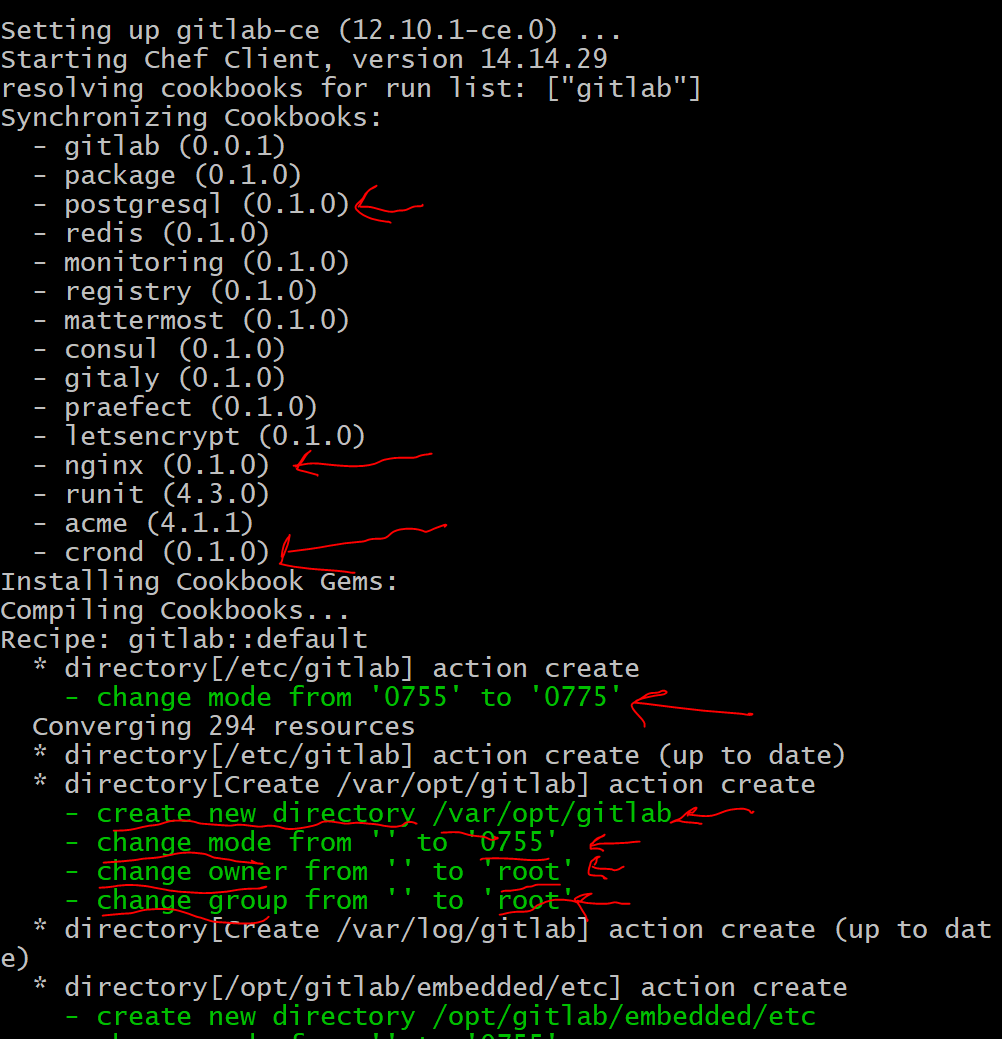
\includegraphics[width=0.8\textwidth]{Images/forClass.PNG}
	\caption{{\small \texttt{Look at the things mentioned in the installer. E.g.
chmod, chgrp, chown, nginx, postgres, crond, etc..}}}
	\label{fig:familiar}
\end{figure}

Now your server works! On the server side, when the install is done you'll see
something like fig~\ref{fig:installDone}. Open a browser on any computer in the world ( almost
anywhere ) and put the ipaddress of your gitlab server in the search bar. A
gitlab webpage will popup. You did that! 

\begin{figure}[h]
\centering
	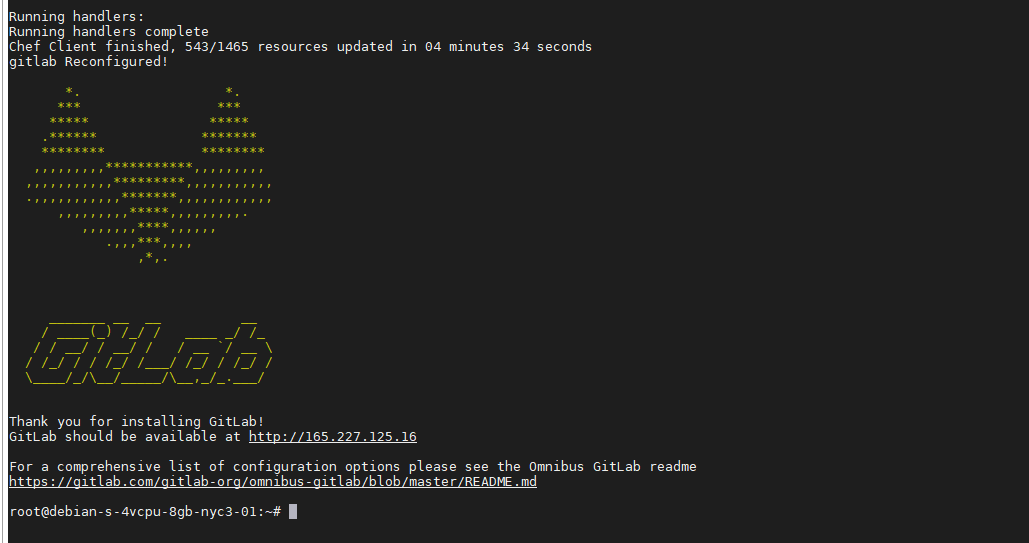
\includegraphics[width=0.8\textwidth]{Images/installDone.PNG}
	\caption{{\small \texttt{What the server shows when installation is done.}}}
	\label{fig:installDone}
\end{figure}


It will ask you to input a new password.

Set the password.

Then log in using the username \textbf{root} and the password you just created.
From here, the website works pretty much like github. You can poke around with
it to learn about it, see fior yourself. 

When your curiosity is satisfied you can destory the droplet on digital ocean.
Remember you're paying mega bucks for this thing. Best thing to do would
probably be find a crappy old pc, stick 8gb ram in it, install debian + gitlab
and then run the server from your house. Or look for a cheaper cloud provider.
Digital ocean is dead cheap to get started with - a bare bones machine for 5
bucks. I'm not sure how economical it is for larger projects, you'd need to do
your own research. Already for ths 8gb machine which we'll rarely use youre
paying 40 a month, that's way too much for my taste, I dont know about yours.


\subsection{ERRNOMEM}

I wanted to see how strict the requirememts were fpr this server. Gitlab says
8gb memory. I tried to run it on a 5 dollar server with 1GB ram. the installer
fails showing a low memory error. Try for yourself! The error I got is shown in
fig~\ref{fig:noMem}.

\begin{figure}[h]
\centering
	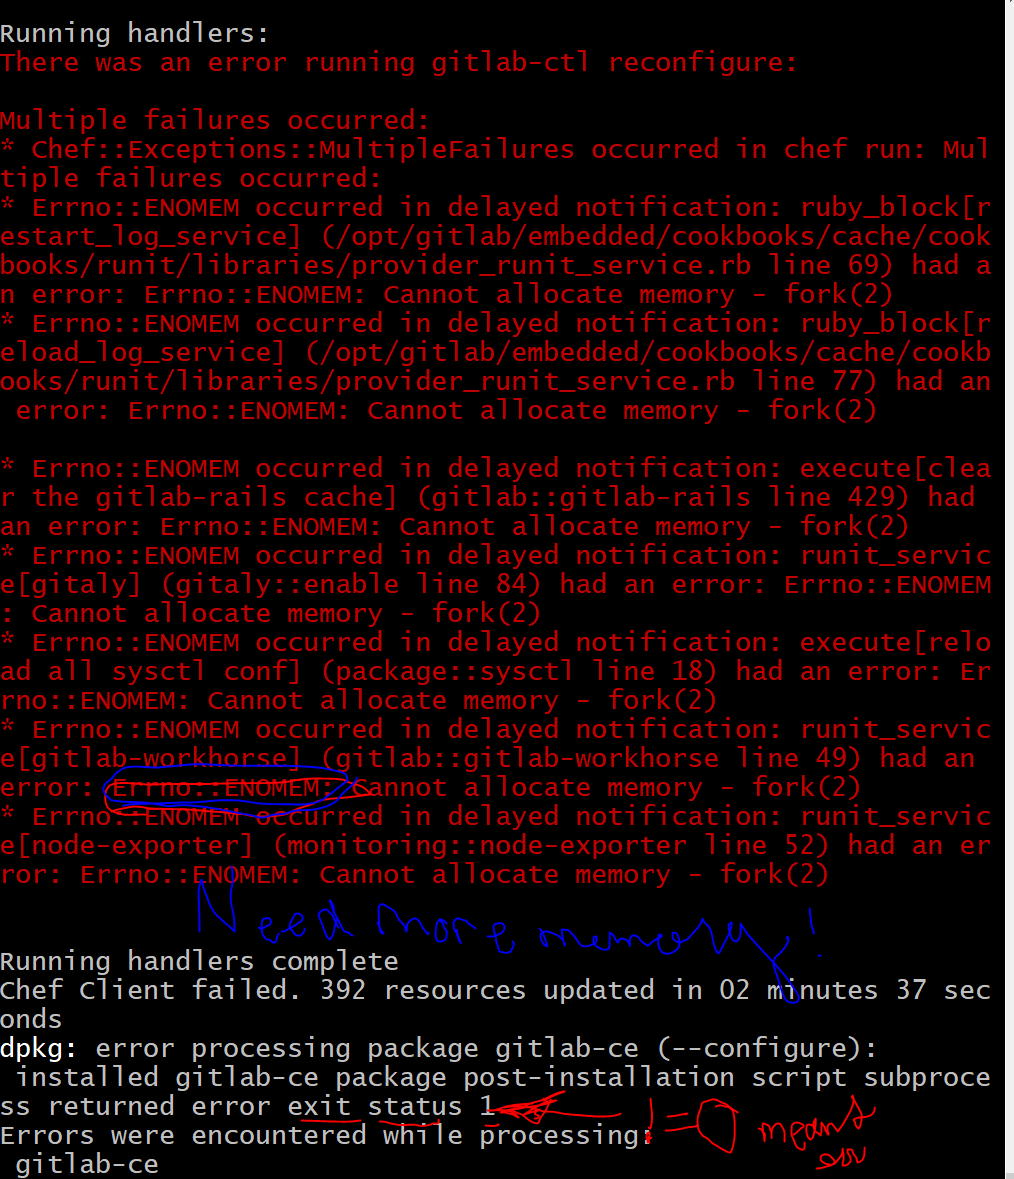
\includegraphics[width=0.8\textwidth]{Images/nomemerror.PNG}
	\caption{{\small \texttt{Can't install gitlab with only 1GB mem.}}}
	\label{fig:noMem}
\end{figure}

To get around this I tried giving a large amount of swap space, 4GB.
Just as we did before. Open a terminal and:

\begin{lstlisting}
root@machine$ fallocate -l 4GB /swapfile
root@machine$ chmod 600 /swapfile
root@machine$ mkswap /swapfile
root@machine$ swapon /swapfile
\end{lstlisting}

and add the following to your /etc/fstab file:

\begin{verbatim}
/swapfile swap swap defaults 0 0
\end{verbatim}


Now if you rerun the installation steps, gitlab will successfully install thanks
to the swap space. \textbf{This will be the slowest website you've ever used. It
will be unusable. This was just done as an experiment and I thought you'd like
to see swapspace in action since we discussed it a few weeks ago.}

\section{Final Interesting Topic 1: \textit{join}}

\begin{center}
\url{https://www.bsdnow.tv/306}
\end{center}

Refer to the "BSD Now" Podcast Episode 306: Comparing Hammers. Listen to around
21 minutes in. Discussion of join, awk, grep, command line relational database
on BSD. Pretty cool stuff you could understand now! Also note that right before
this they are talking about Hammer vs. Hammer 2, which are file systems types on
BSD ( not available on Linux )

Do you remember what are some common Linux file system types?

Note at 21:40 they say Postgres Server! You made one of those! You can listen to
hte pro BSD podcasts now and confidently say to yourself that you've done the
things they are talking about.

\subsection{Back to \textit{join}}
I gave two files you can use to test this cool command. One is
\textit{students.sorteddata}

\lstinputlisting{students.sorteddata}

and the other is \textit{roomnumber.sorteddata}

\lstinputlisting{roomnumber.sorteddata}

And note that we can do an inner join on them using the \textit{join} command!

\begin{lstlisting}
melvyn@laptop$ join -1 2 -2 1 -t"," students.sorteddata roomnumber.sorteddata
biology,katyusha,202
chemistry,igor,106
math,boris,101
math,svetlana,101
\end{lstlisting}

See?? It does an inner join!

If you use the unsorted data files in the repo you will see that it complains,
it wants the data sorted.

\subsection{\textit{join} and \textit{awk}}
In the podcast they go on to say you can use awk and grep to do your SELECT *
WHERE X = Y operations you know from our brief discussion of SQL when we set up
the postgres server. Can you do the join and then use awk to print the lines
where the subject is math?

\begin{figure}[h]
  \centering
    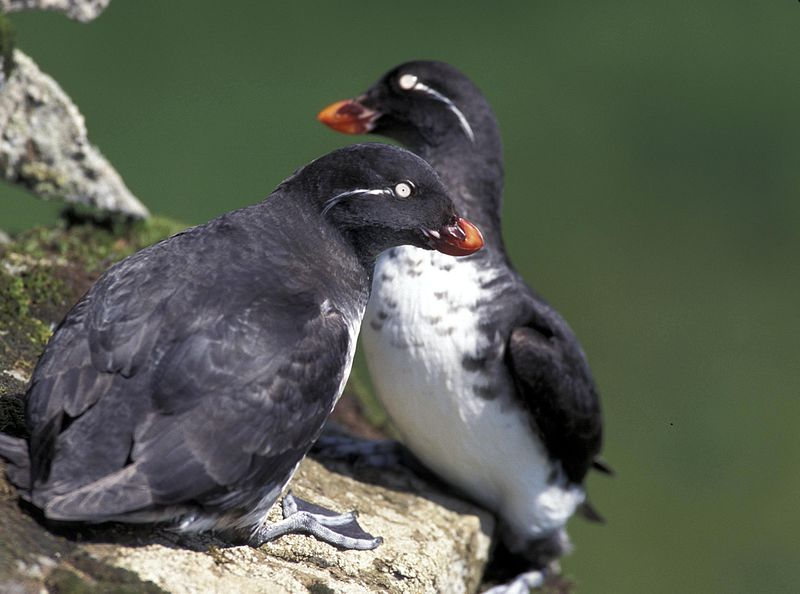
\includegraphics[width=0.8\textwidth]{auk.jpg}
  \caption{This bird is an auk. The language is called AWK because the language creators are Aho,
Weinberger and Kernighan ( A. W. K. ), and `AWK' sounds like `auk'.}
\end{figure}



\section{Final Interesting Topic 2: Linux on an Atmel Microcontroller}
You are computer science majors, or techy types - look at the cool stuff your
peers are working on:
\url{https://dmitry.gr/index.php?r=05.Projects&proj=07.%20Linux%20on%208bit}
This fellow got Linux ( which expects a 32bit or 64bit architecture to run ) to
run on a teensy 8 bit Atmel microcontroller. This guy gathered a bunch of
electronics pieces and soldered them onto a circuit board. He then programmed a
CPU emulator in C that tricked Linux into thinking the 8 bit microcontroller 
was actually 32 bits. Then he installed a carefully chosen Linux image onto his
little computer, and then it worked! 
It's just an amazing display of hardware and software knowledge that this
creative person  pulled together to do something that others said was
impossible. 

This guy, Dmitry Grinberg, had a full time job, family and a bunch of hobbies
while he did this.

\section{Keep Learning and Keep Doing Cool Stuff}
Read lots of books, learn a few programming languages, do some projects, it's
good for you.
\end{document}
